\phantomsection
% \addcontentsline{toc}{chapter}{Appendices}

% The \appendix command resets the chapter counter, and changes the chapter numbering scheme to capital letters.
%\chapter{Appendices}
 \appendix
\chapter{Multimodal Correlations}
\begin{figure}
    \centering
    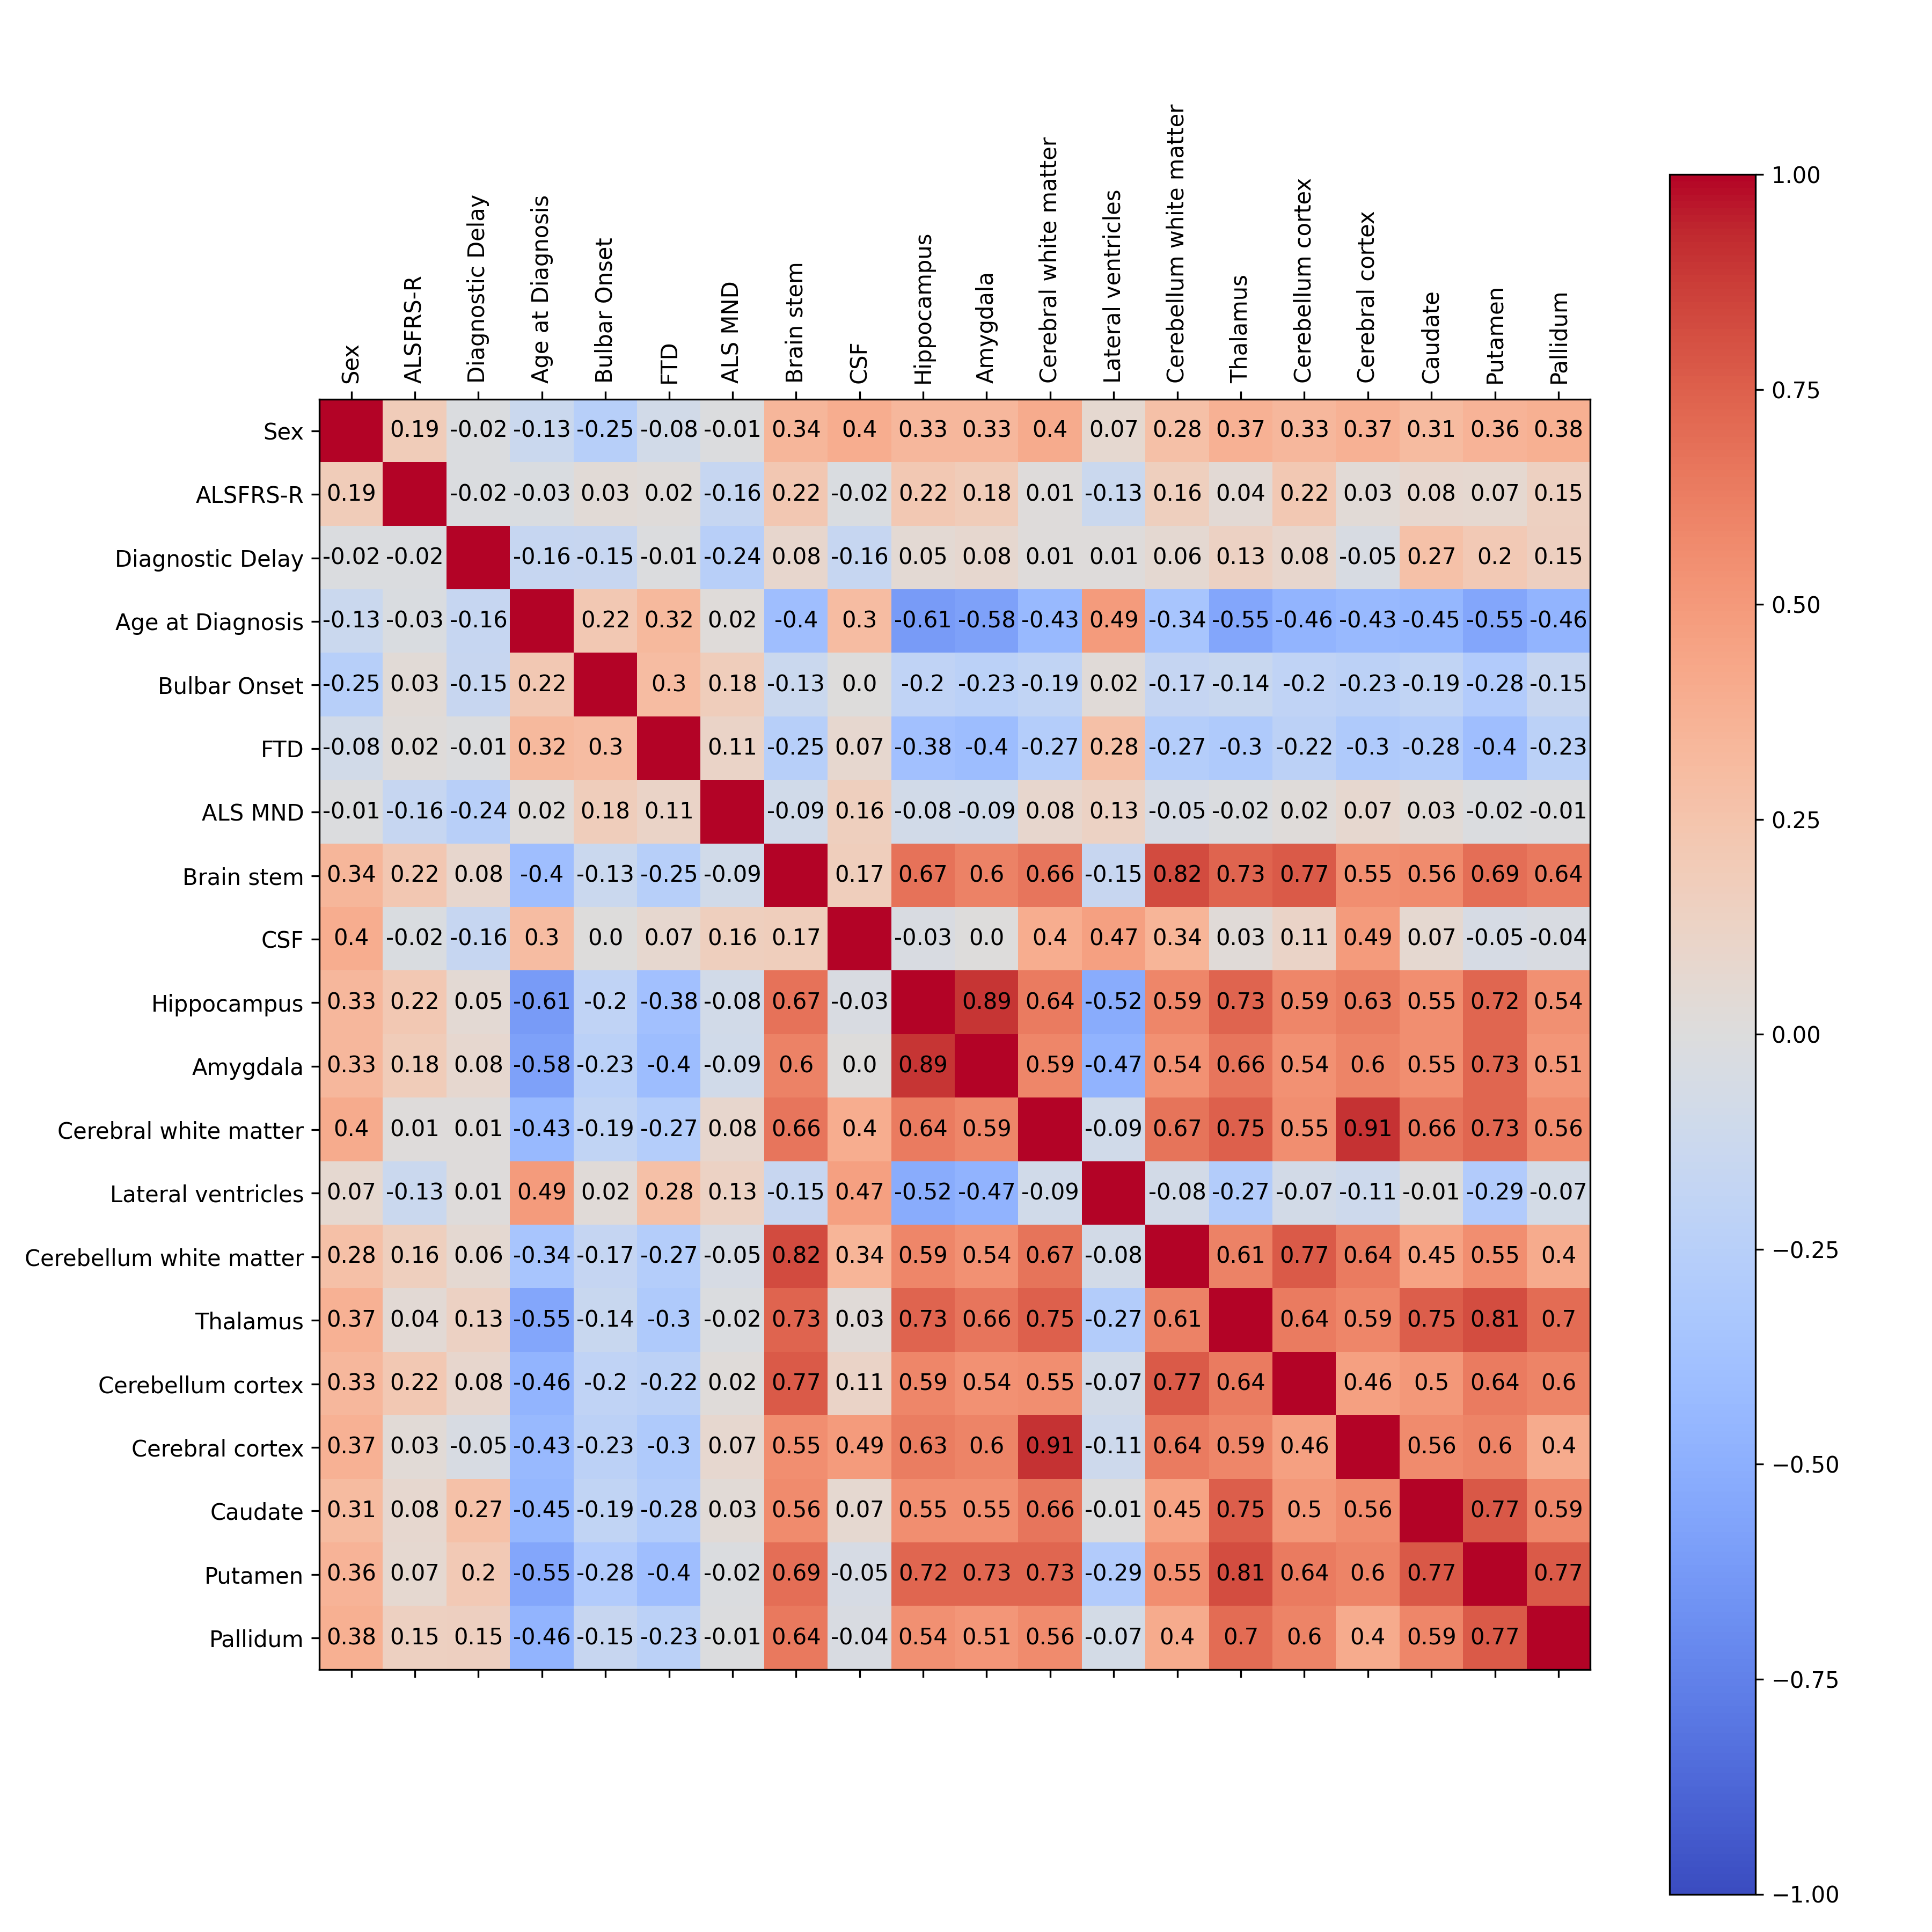
\includegraphics[width=\textwidth]{figures/multimodal_correlation}
    \caption{Correlations of all of the features included in the multimodal multivariable Cox proportional hazards model in Chapter~\ref{cox_proportional_hazards_model}.}
    \label{fig:multimodalcorrelations}
\end{figure}

\chapter{Fusion Model Architectures}
\label{appendix:fusion_model_architectures}

%(stuff)
%
%\chapter{Another Appendix About Things}
%\label{appendixlabel2}
%(things)
%
%\chapter{Colophon}
%\label{appendixlabel3}
%\textit{This is a description of the tools you used to make your thesis. It helps people make future documents, reminds you, and looks good.}
%
%\textit{(example)} This document was set in the Times Roman typeface using \LaTeX\ and Bib\TeX , composed with a text editor.
 % description of document, e.g. type faces, TeX used, TeXmaker, packages and things used for figures. Like a computational details section.
% e.g. http://tex.stackexchange.com/questions/63468/what-is-best-way-to-mention-that-a-document-has-been-typeset-with-tex#63503

% Side note:
%http://tex.stackexchange.com/questions/1319/showcase-of-beautiful-typography-done-in-tex-friends
